% =====================================================================
%  Kleines Symbol der Oberfräse für den Kopf der Betriebsanweisung
%  (\BAsetup{bildcode=...}). Ohne zeichnungen/stil.tex lauffähig.
%  Selbst gezeichnet.
% =====================================================================
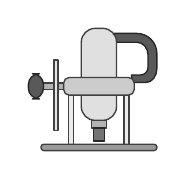
\begin{tikzpicture}[x=0.16mm, y=0.16mm, line width=0.5pt, line join=round]
  % Führungssäulen und Stiel des Drehknopfs
  \draw[fill=black!8, draw=black!75] (-24,5) rectangle (-20,50) (20,5) rectangle (24,50);
  \draw[fill=black!30, draw=black!75] (-44,48.5) rectangle (-28,53.5);
  % Drehknopf und Handgriff
  \draw[fill=black!65, draw=black!85, rounded corners=4] (-56,41) rectangle (-44,61);
  \draw[fill=black!65, draw=black!85] (12,93) -- (30,93) to[out=0,in=90] (46,77) -- (46,65)
    to[out=-90,in=0] (37,54) -- (26,54) -- (26,60) -- (33,60)
    to[out=0,in=-90] (39,66) -- (39,76) to[out=90,in=0] (30,86) -- (12,86) -- cycle;
  % Motor, Spannmutter, Fräser
  \draw[fill=black!12, draw=black!75, rounded corners=5] (-14,24) rectangle (14,97);
  \draw[fill=black!30, draw=black!75] (-6,18) rectangle (6,24);
  \draw[fill=black!55, draw=black!85] (-4.5,7.5) rectangle (4.5,18);
  % Motorträger, Tiefenanschlag, Frästisch
  \draw[fill=black!20, draw=black!75, rounded corners=2] (-28,44) rectangle (28,58);
  \draw[fill=black!10, draw=black!75] (-35.5,16) rectangle (-32.5,72);
  \draw[fill=black!40, draw=black!75, rounded corners=1] (-46,0) rectangle (46,5);
\end{tikzpicture}
